\documentclass{beamer}

\usepackage{amsmath}
\usepackage{amssymb}
\usepackage{amstext}
\usepackage{amsthm}
\usepackage{palatino}
\usepackage{subfigure}
\usepackage{graphicx}
\usepackage{hyperref}
\hypersetup{colorlinks=false}
\usepackage{url}
\usepackage[utf8]{inputenc} 

\newcommand{\Z}{\mathbb{Z}}
\newcommand{\R}{\mathbb{R}}
\newcommand{\N}{\mathbb{N}}
\newcommand{\lam}[2]{\lambda#1.#2}
\newcommand{\BETA}{\boldsymbol\beta}
\newcommand{\barrow}{\rightarrow_\beta}
\newcommand{\Barrow}{\barrow^*}
\newcommand{\I}{\textsf{\textbf{I}}}
\newcommand{\W}{\textsf{\textbf{W}}}

% Bruges til Python-kode.
\newcommand{\pycode}[1]{\textbf{\texttt{#1}}}


\begin{document}
\title{Visualization of $\beta$-reduction Graphs in the Lambda Calculus}   
\author{Niels Bjørn Bugge Grathwohl og Jens Duelund Pallesen} 
\date{13. august 2010} 

\frame{\titlepage}

\frame{\frametitle{Indhold}\tableofcontents} 


\section{Introduktion}
\frame{\frametitle{Introduktion} 
\begin{itemize}
	\item Der findes visualiseringer af lambda kalkylen generelt, men ingen visualiseringer af reduktionsgrafer.
	\item Disse visualiseringer er forskellige måder at tegne syntakstræer for en term på, på forskellige stadier
	i en kæde af reduktioner af den term. 
	\item Programmet udvilket i dette projekt illustrerer de forhold der gælder mellem
	termer ved $\beta$-reduktion, ved at lægge dem ud som en graf.
	\item Produktet er udviklet med henblik på forskere og undervisere inden for området.
\end{itemize}
}


\section{Design}
\frame{\frametitle{Design} 
\begin{itemize}
	\item Opdelt design, gør det muligt at udskifte individuelle dele uafhængigt af hinanden.
	\item Designet gør det let at udvide med nye tegnealgoritmer.
	\item Multiplatform (Python og GTK).
\end{itemize} 
}

\subsection{Grafgenerator}
\frame{\frametitle{Design: Grafgenerator} 
\begin{itemize}
	\item Parse $\rightarrow$ Find redexer $\leftrightarrow$ Reducér
	\item Parseren oversætter en tekststreng til en interne DAG-repræsentation af en term.
	\item På denne repræsentation anvendes en funktion der returnerer alle positioner på redexer i termen.
	\item Denne liste løbes igennem, og redexerne reduceres til deres kontrakta.
	\item Hvert uset kontraktum tilføjes reduktionsgrafen.
	\item Forbindelser mellem termen der reduceres samt dets kontrakta indkodes i reduktionsgrafen, 
	og næste term i grafen tages under behandling.
	\item For at imødekomme problemet med uendeligt store grafer, fungerer grafgeneratoren
	som en iterator, der returnerer en stadigt mere ``komplet'' reduktionsgraf.
	% \item Generering af tilfældige grafer
\end{itemize} 
}

\subsection{Graftegner}
\frame{\frametitle{Design: Graftegner} 
\begin{itemize}
	\item GraphViz -- Tilbyder en række tegnealgoritmer.
	\item Majorization -- Vores egen implementation af en tegnealgoritme, som tilbyder
	ekstra fleksibilitet i forhold til GraphViz's tegnealgoritmer (animering, tweaks).
	\item PyGTK -- Brugt til GUI pga. god understøttelse samt at det er enkelt at benytte.
	\item Python Widgets -- Brugt til at binde de forskellige GUI elementer sammen.
\end{itemize} 
}

\subsection{Graftegner 2}
\frame{\frametitle{Design: Grafiske elementer}
\begin{itemize}
	\item ``Menige'' knuder tegnes som sorte cirkler.
	\item Normalformer er tegnet som store røde cirkler.
	\item Starttermen er fremhævet som en mellemstor, grøn cirkel.
	\item Hvis brugeren har valgt det fremhæves den ``aktive'' knude som en
	mellemstor, mørkegrøn cirkel.
	\item Selvrefererende knuder tegnes som røde firkanter.
\end{itemize}
}

\subsection{GUI}
\frame{\frametitle{Design: GUI} 
\begin{itemize}
	\item Ikke en GUI opgave.
	\item Dog er et minimum af GUI en nødvendighed for at kunne anvende programmet
	\item Enkel GUI
\end{itemize}
\begin{figure}[htbp!]
	\centering
		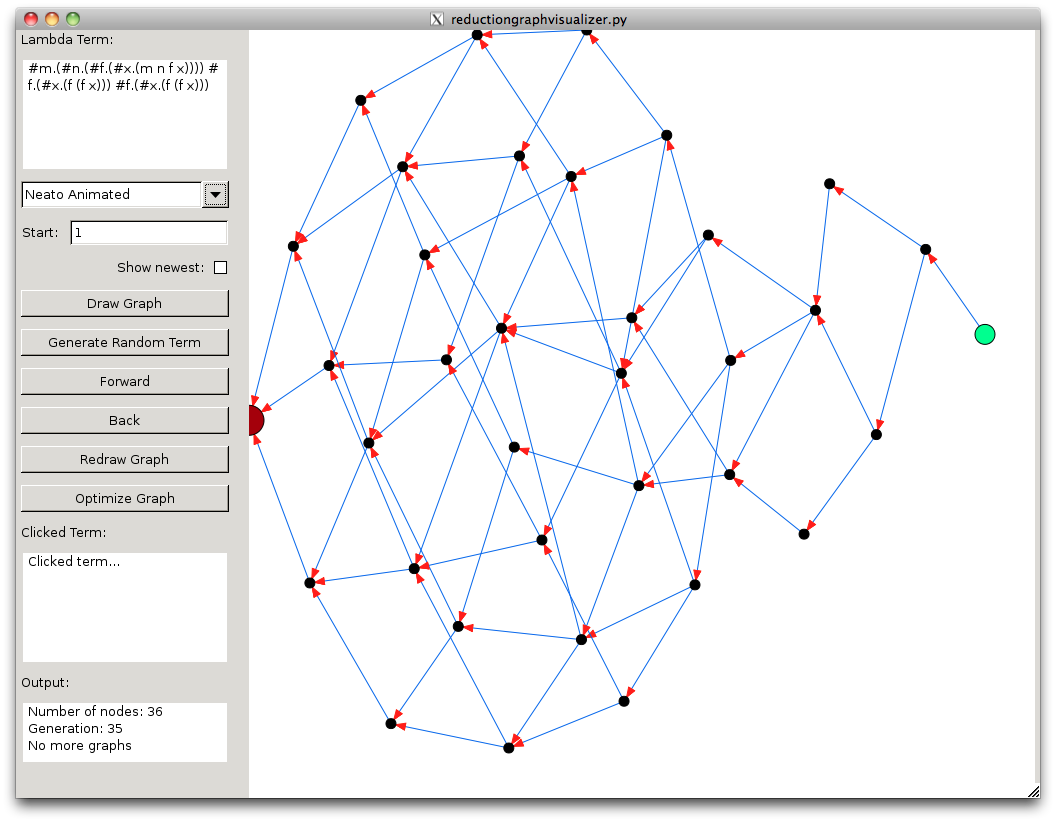
\includegraphics[height=2in]{screen.png}
	\label{fig:screen}
\end{figure}
}

\section{Eksempler}
\frame{\frametitle{Eksempler} 
\begin{itemize}
	\item Predecessor og Successor.
	\item Addition, multiplikation og potens.
	\item Hypercube.
	\item Association.
	\item Cons.
\end{itemize} 
}

\subsection{Predecessor og Successor}
\frame{\frametitle{Predecessor og Successor} 
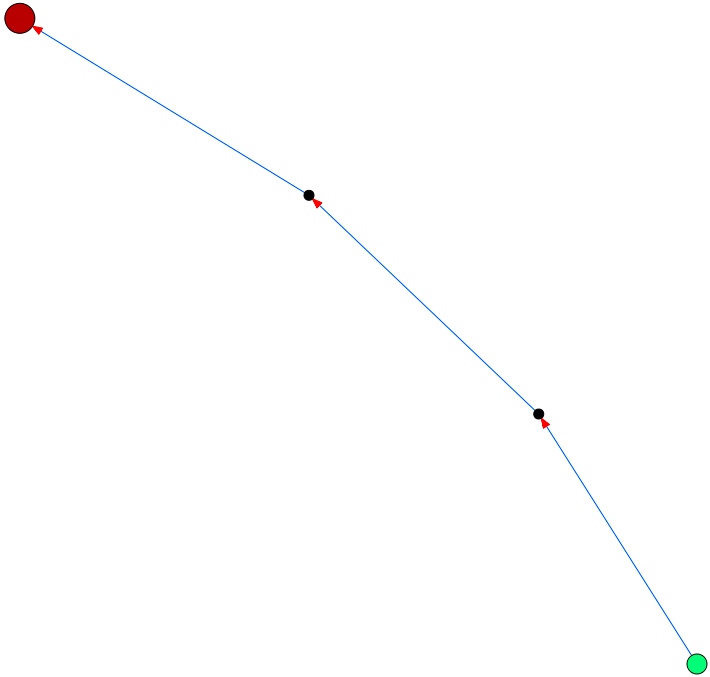
\includegraphics[height=2in]{Succ5_NEATO.png}
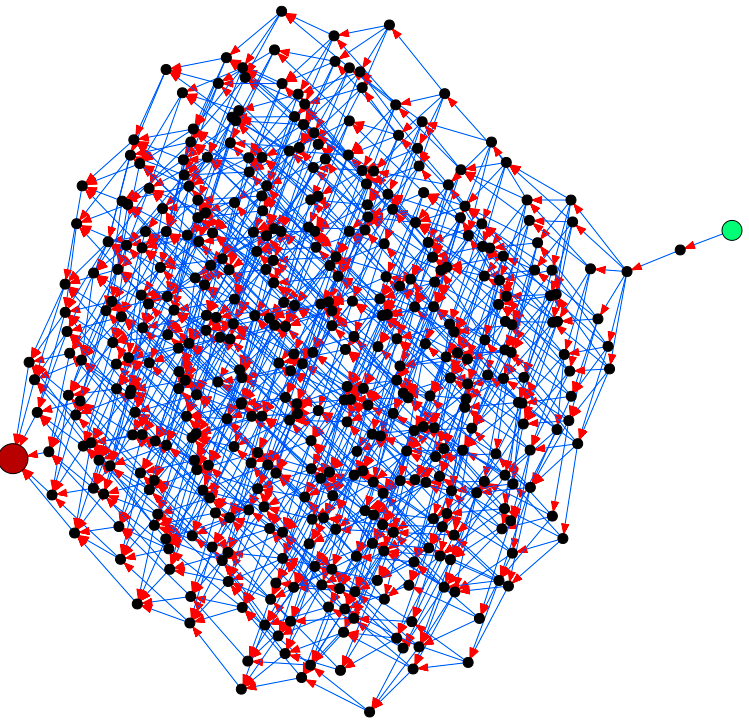
\includegraphics[height=2in]{Pred5_NEATO.png}
}

\subsection{Addition, multiplikation og potens}
\frame{\frametitle{Addition, multiplikation og potens}
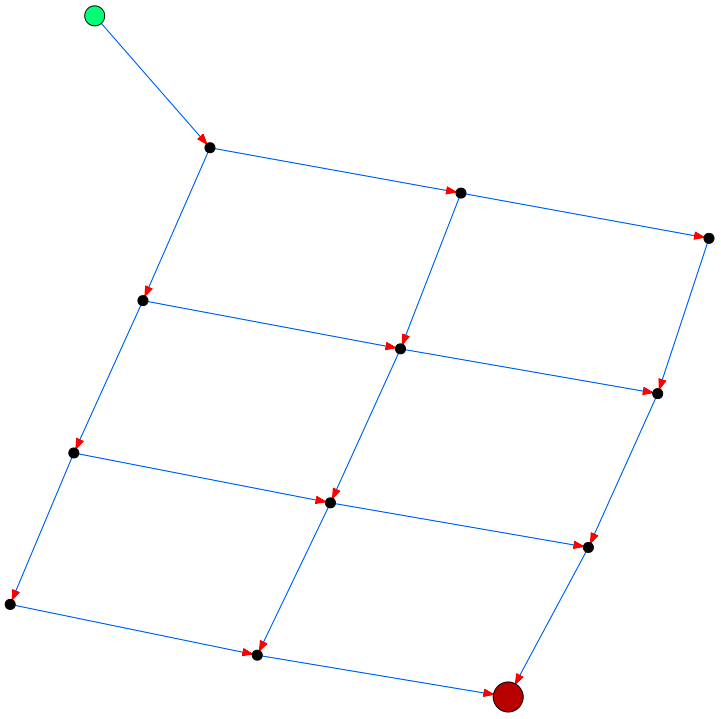
\includegraphics[height=1.5in]{Sum22_NEATO.png}
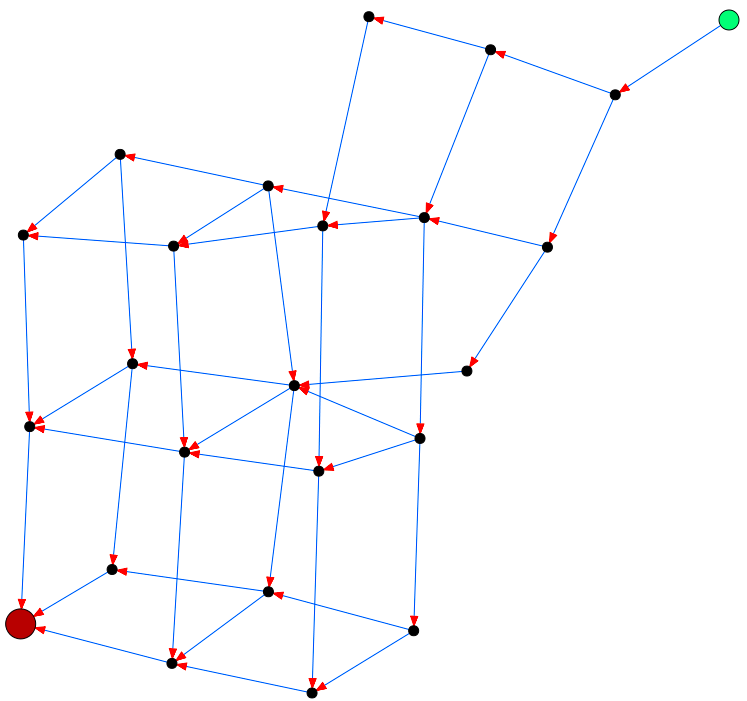
\includegraphics[height=1.5in]{Prod22_NEATO.png}
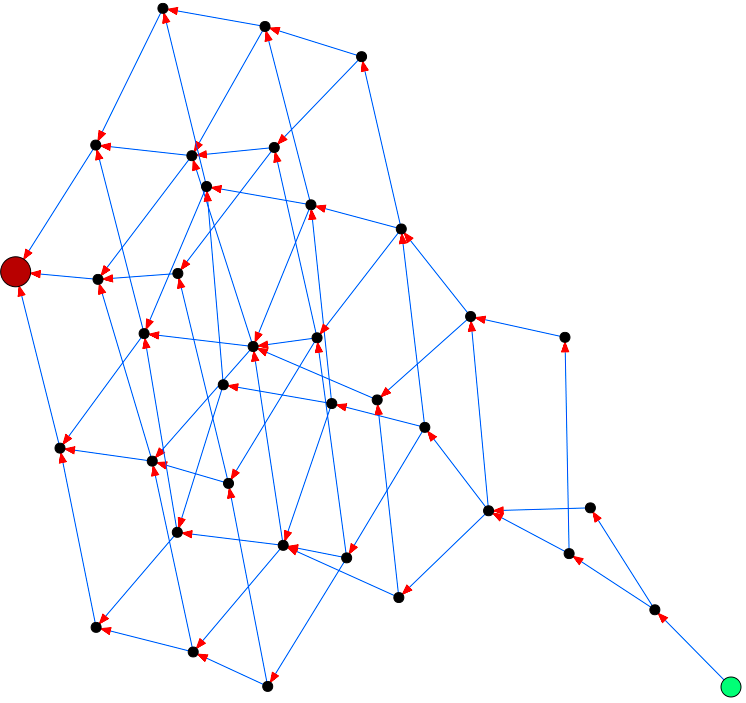
\includegraphics[height=1.5in]{Exp22_NEATO.png}
}

\subsection{Hypercube}
\frame{\frametitle{Hypercube ($((\lam{x_1}{x_1}) f)\hdots((\lam{x_n}{x_n}) f)$)}
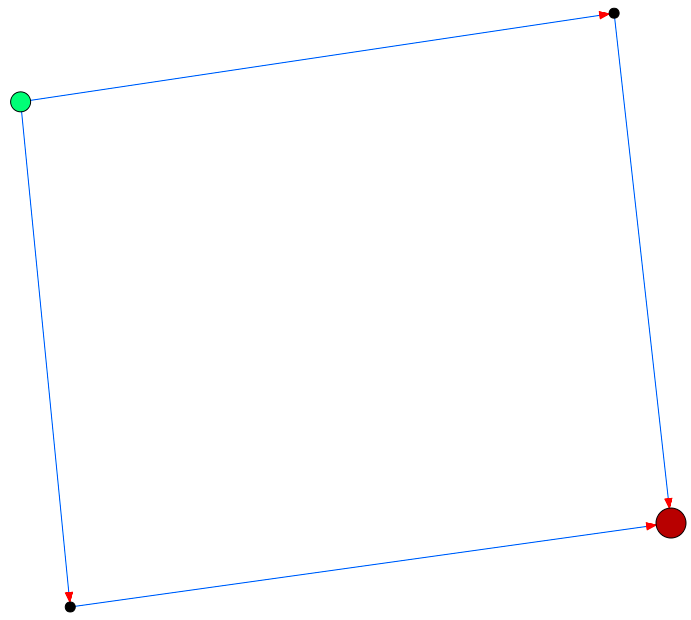
\includegraphics[height=1.5in]{Cube2d_NEATO.png}
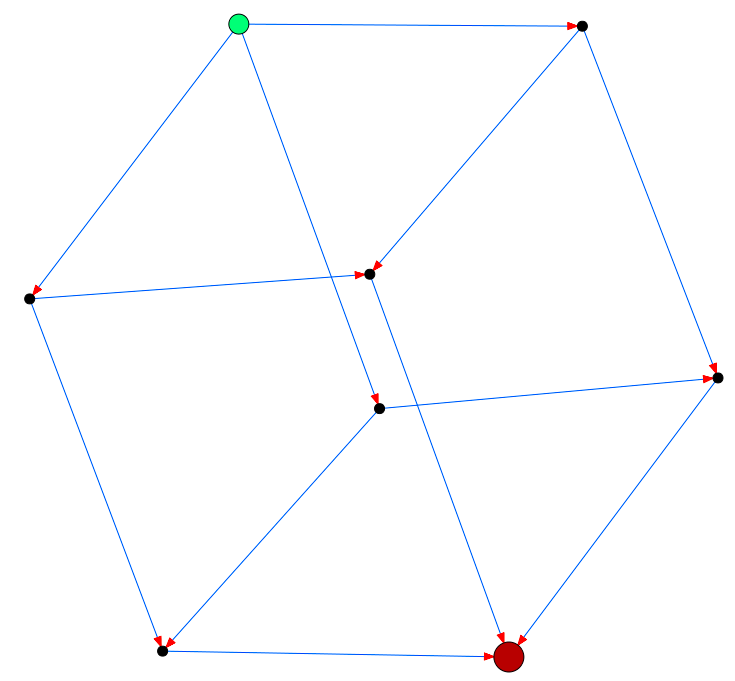
\includegraphics[height=1.5in]{Cube3d_NEATO.png}
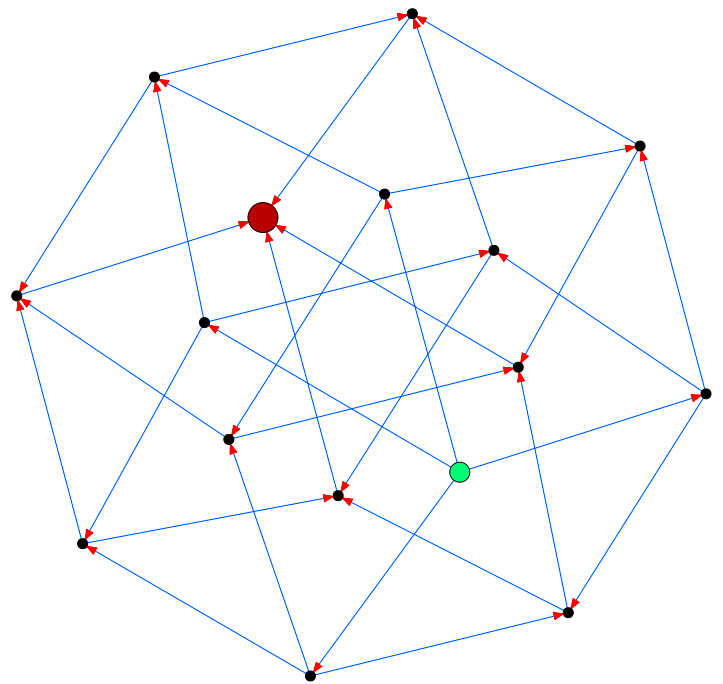
\includegraphics[height=1.5in]{Cube4d_NEATO.png}
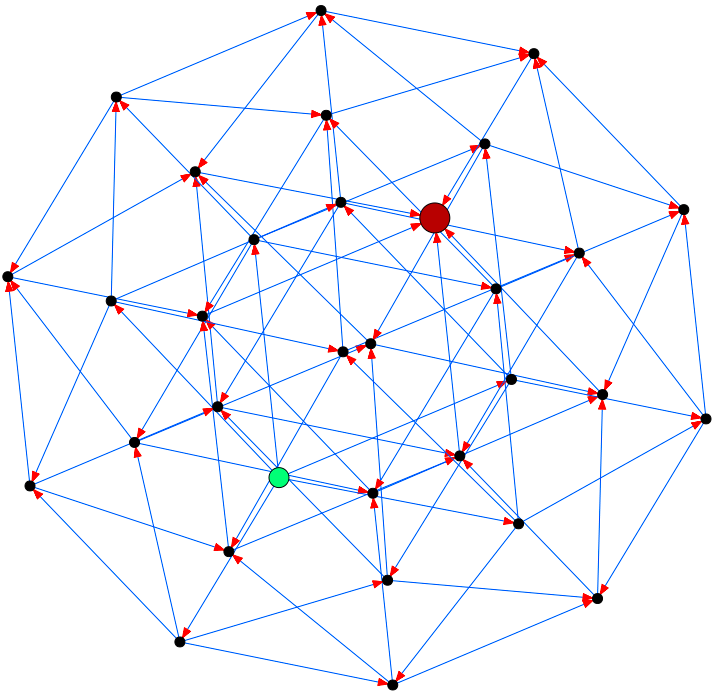
\includegraphics[height=1.5in]{Cube5d_NEATO.png}
}

\subsection{Association}
\frame{\frametitle{Association}
\begin{figure}[htbp!]
	\subfigure[$\omega_3 \omega_3 \omega_3 \omega_3$]{
		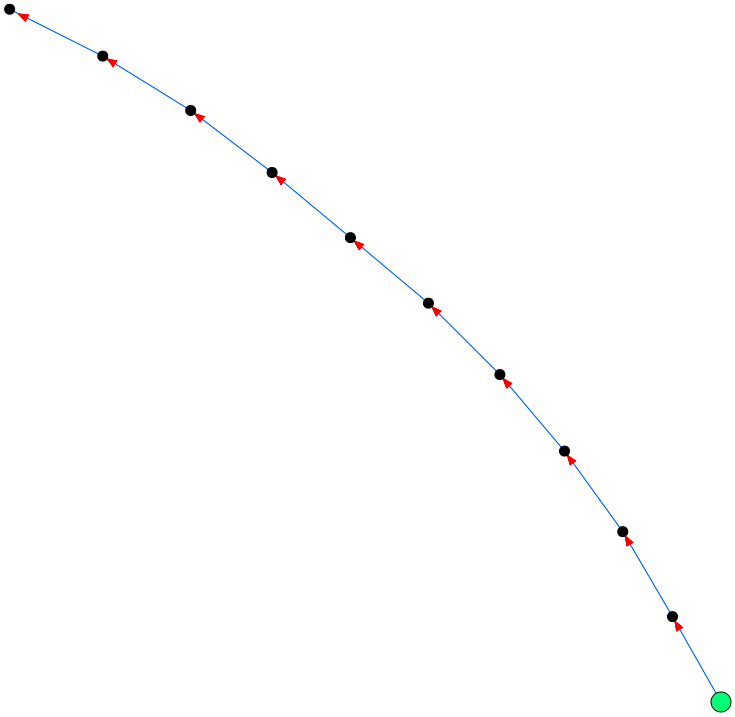
\includegraphics[height=1.2in]{Snake_2_NEATO.png}
	}
	\subfigure[$\omega_3 \omega_3 (\omega_3 \omega_3)$]{
		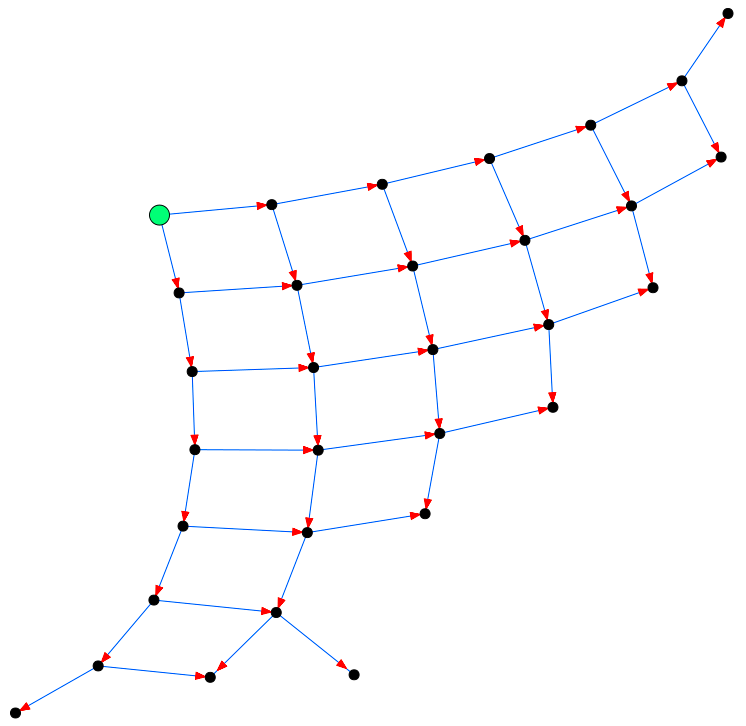
\includegraphics[height=1.2in]{Snake_3_NEATO.png}
	}
	\subfigure[$\omega_3 (\omega_3 (\omega_3 \omega_3))$]{
		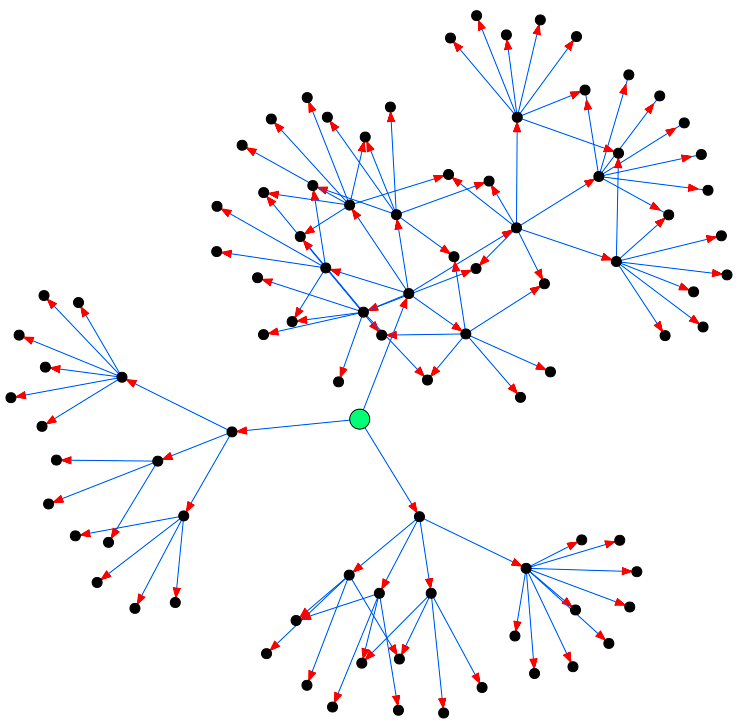
\includegraphics[height=1.2in]{Snake_4_NEATO.png}
	}
\end{figure}

}

\subsection{Cons}
\frame{\frametitle{Cons}
\begin{figure}[htbp!]
	\subfigure[(2,3)]{
		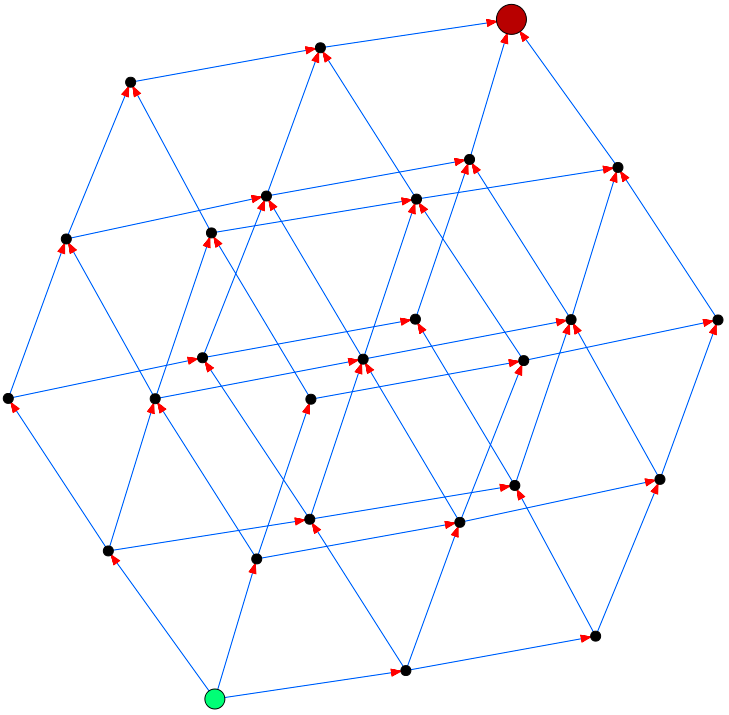
\includegraphics[height=1.2in]{Cons23_NEATO.png}
	}
	\subfigure[(4,4)]{
		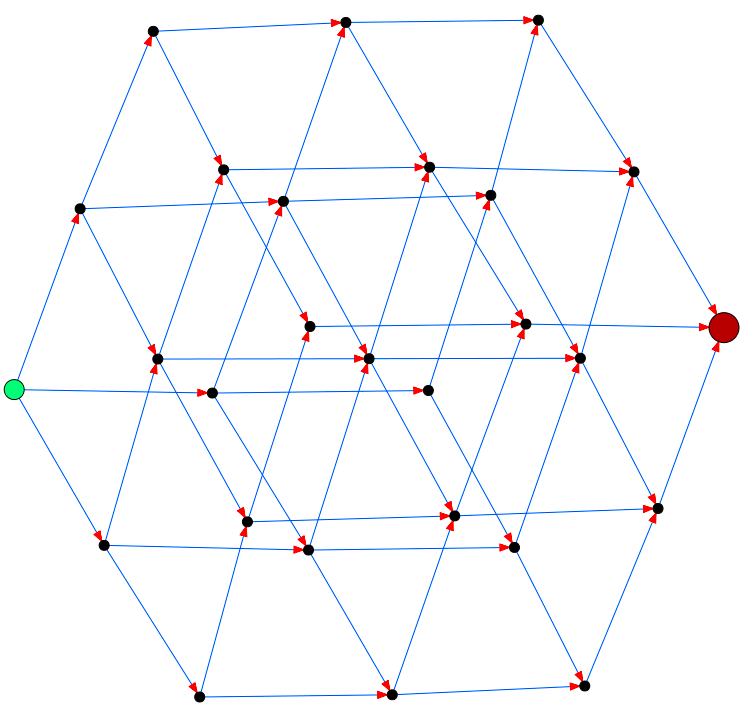
\includegraphics[height=1.2in]{Cons44_NEATO.png}
	}
	\subfigure[(5,0)]{
		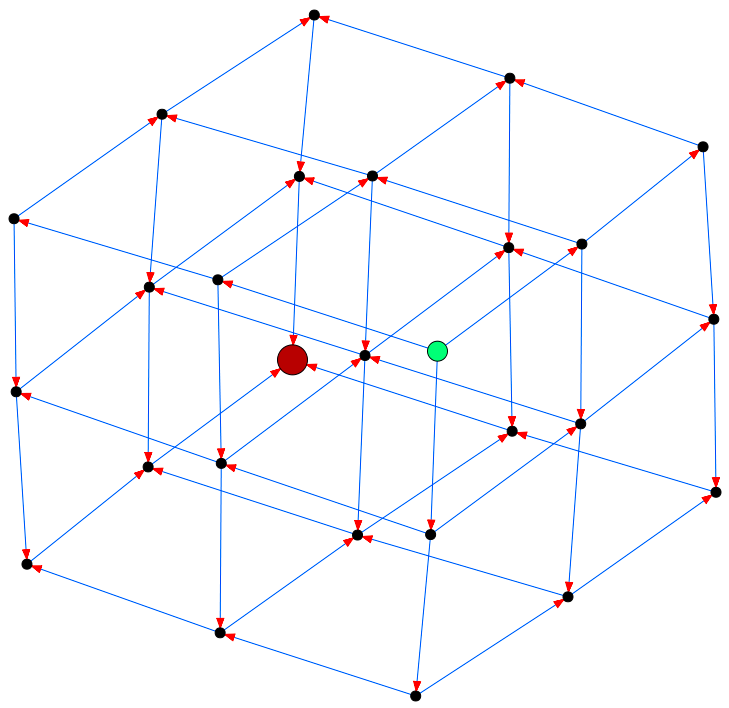
\includegraphics[height=1.2in]{Cons50_NEATO.png}
	}
\end{figure}
}

\subsection{Forskellige tegnealgoritmer}
\frame{\frametitle{Forskellige tegnealgoritmer}
\begin{figure}[htbp!]
	\subfigure[Circo]{
		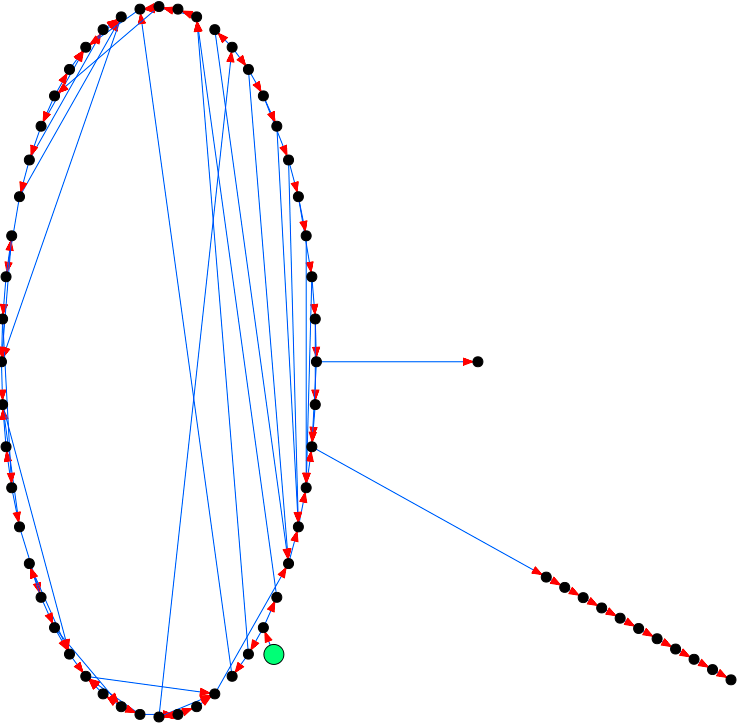
\includegraphics[width=1.2in]{Ycomb_3_CIRCO.png}
	}
	\subfigure[Dot]{
		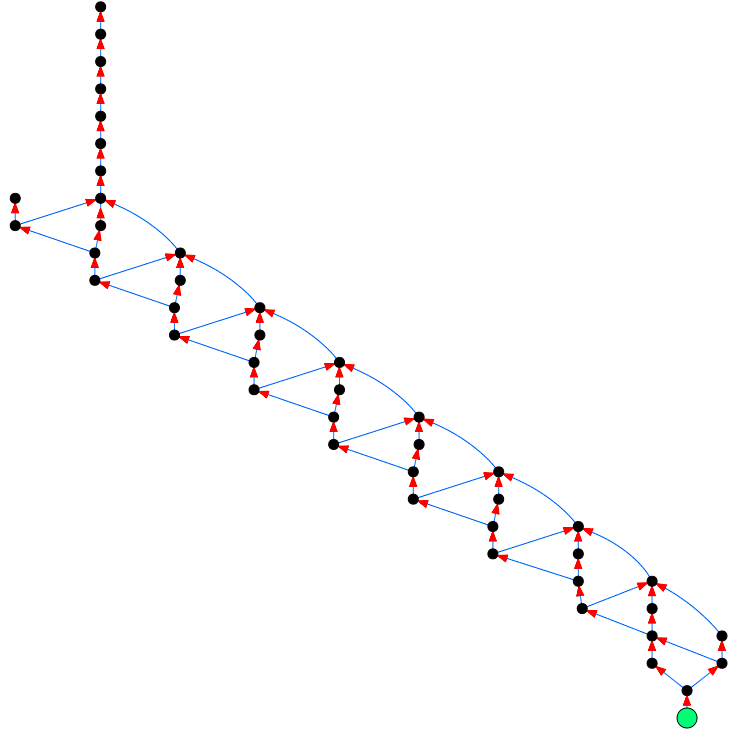
\includegraphics[width=1.2in]{Ycomb_3_DOT.png}
	}
	\subfigure[Fdp]{
		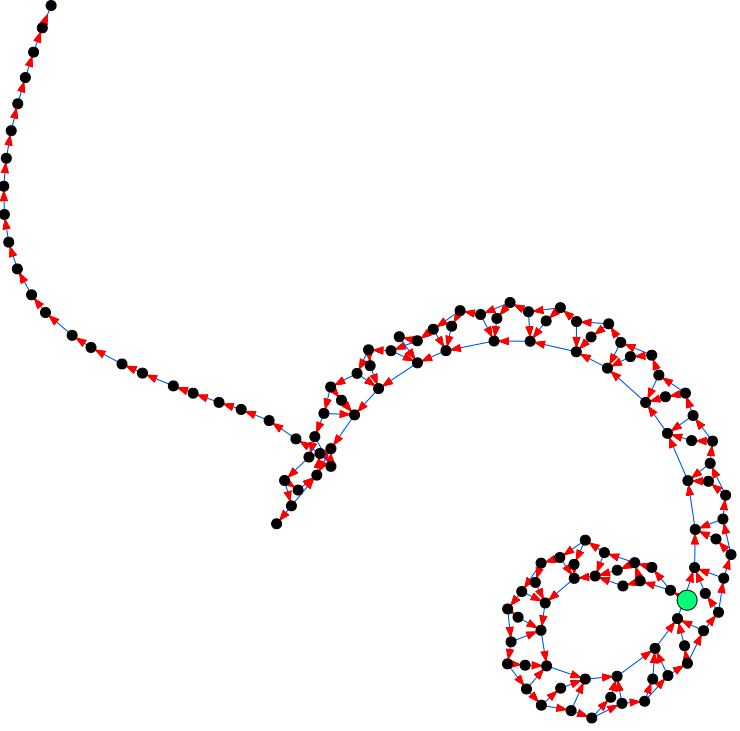
\includegraphics[width=1.2in]{Ycomb_3_FDP.png}
	}
	\subfigure[Neato Animated]{
		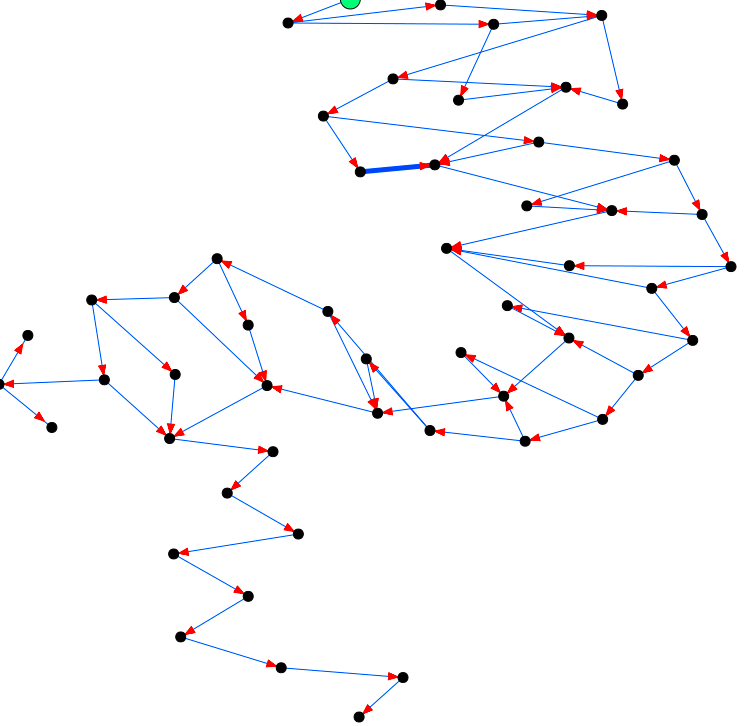
\includegraphics[width=1.2in]{Ycomb_3_MAJOR.png}
	}
	\subfigure[Neato]{
		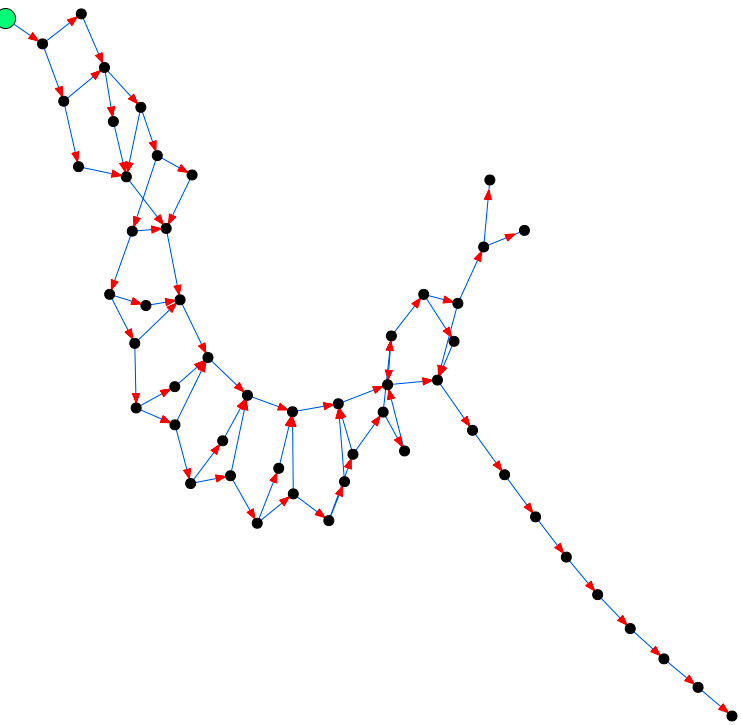
\includegraphics[width=1.2in]{Ycomb_3_NEATO.png}
	}
	\subfigure[Twopi]{
		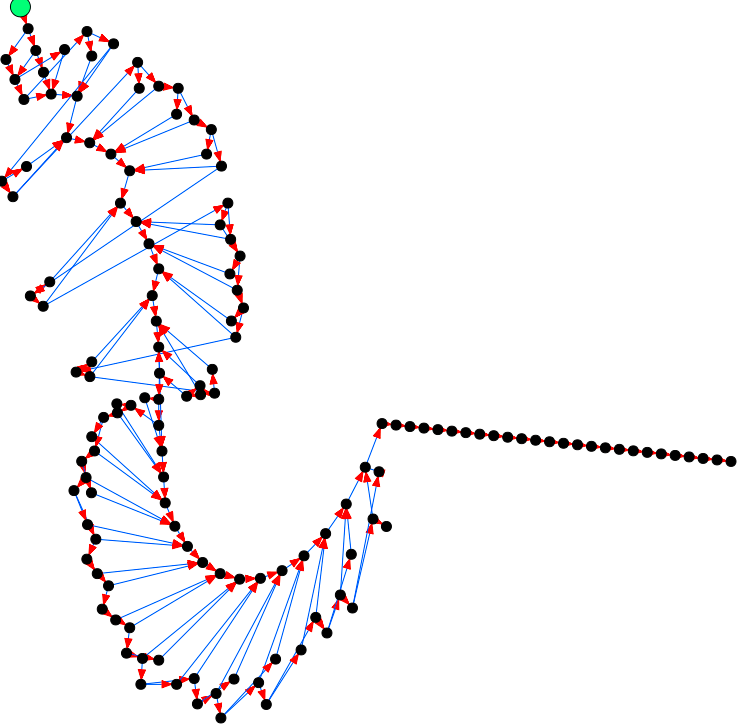
\includegraphics[width=1.2in]{Ycomb_3_TWOPI.png}
	}
\end{figure}
}

\section{Performance}
\frame{\frametitle{Performance}
\begin{itemize}
	\item Neato giver bedste all-round resultater mht. brugbarhed.
	\item Benchmarks (kørsler af layoutalgoritmerne uden GUI og uden at tegne grafen):
\end{itemize} 
\begin{center}
	\begin{tabular}{| c | c | c | c | c | c |}
		\hline
		\multicolumn{6}{|c|}{Lambda Term: Predecessor til 4} \\
		\multicolumn{6}{|c|}{Generationsnummer: 300} \\
		\hline Neato Animated & Circo & Dot & Neato & TwoPi & Fdp \\
		\hline 4.36 s & 310.44 s & 0.91 s & 1.11 s & 0.23 s & 10.90 s \\
		\hline
	\end{tabular}
\end{center}
\begin{center}
	\begin{tabular}{| c | c | c | c | c | c |}
		\hline
		\multicolumn{6}{|c|}{Lambda Term: $2^2$} \\
		\multicolumn{6}{|c|}{Generationsnummer: 35} \\
		\hline Neato Animated & Circo & Dot & Neato & TwoPi & Fdp \\
		\hline 0.05 s & 0.12 s & 0.04 s & 0.05 s & 0.04 s & 0.09 s \\
		\hline
	\end{tabular}
\end{center}
}

\section{Fremtidigt arbejde}
\frame{\frametitle{Fremtidigt arbejde}
\begin{itemize}
	\item Udbygge med flere graftegnealgoritmer.
	\item Udbygge med flere reduktionssystemer end lambda kalkyle.  
	\item OpenGL omskrivning (3D, zooming, etc.)
	\item Highlighting af forskellige reduktionsstrategiers ``stier'' gennem reduktionsgrafen.
	\item Multitrådet.
	\item Eksport/import af grafer.
	\item Reel brugertest.
\end{itemize} 
}

\section{Konklusion}
\frame{\frametitle{Konklusion} 
\begin{itemize}
	\item En 1. version der gør det muligt hurtigt at se komplekse reduktionsgrafer,
	der ville tage lang tid at udregne og tegne i hånden.
	\item Gode udbyggelsesmuligheder.
\end{itemize} 
}

\end{document}

